\documentclass[letterpaper]{article}

\usepackage{graphicx}  %Required
\usepackage{multirow}
\usepackage{amsmath,amsfonts,amssymb}
\usepackage[left=2cm, right=2cm, top=2cm]{geometry}

\title{Supplementary Material:\\Disentangled Representation Learning for\\Non-Parallel Text Style Transfer}


\date{}
\author{}
\begin{document}
\maketitle
\graphicspath{{images/}}

% used for table headers
\newcommand{\tabh}[1]{\multicolumn{1}{c|}{\textbf{#1}}}
% used for the top left cell in a table
\newcommand{\tabc}[2]{\multicolumn{1}{|c||}{\multirow{#1}{*}{\textbf{#2}}}}
% used for denoting the loss symbol with a subscript
\newcommand{\loss}[1]{J_{\text{#1}}}

\renewcommand\thesection{\Alph{section}}

\section{Sentiment Transfer Ablation Tests}
We conducted ablation tests on the Yelp dataset, and show results in Table~\ref{tab:ablation-results}.
With $\loss{VAE}$ only, we cannot achieve reasonable style transfer accuracy by substituting an empirically estimated style vector of the target style.
This is because the style and content spaces would not be disentangled spontaneously with the autoencoding loss alone.
With either $\loss{mul(s)}$ or $\loss{adv(s)}$, the model achieves reasonable transfer accuracy and cosine similarity.
Combining them together improves the transfer accuracy to $90\%$, outperforming previous methods by a margin of $10\%$.
This shows that the multi-task loss and the adversarial loss work in different ways.
Our insight of combining the two auxiliary losses is a simple yet effective way of disentangling latent space.
However, $\loss{mul(s)}$ and $\loss{adv(s)}$ only regularize the style information, leading to gradual drop of content preserving scores.
Then, we have another insight of introducing content-oriented auxiliary losses, $\loss{mul(c)}$ and $\loss{adv(c)}$, based on BoW features, which regularize the content information in the same way as the style information.
By incorporating all these auxiliary losses, we achieve high transfer accuracy, high content preservation, as well as high language fluency.

\begin{table}[ht]
	\centering
	\begin{tabular}{| l || c | c | c | c || c |}
		\hline
		\tabc{1}{Objectives}                                                            & \textbf{STA}  & \textbf{CS}   & \textbf{WO}   & \textbf{PPL} & \textbf{GM}   \\
		\hline\hline
		$\loss{AE}$                                                                     & 0.11          & \textbf{0.94} & 0.47          & 40           & 0.11          \\ \hline
		$\loss{AE}$, $\loss{mul(s)}$                                                    & 0.77          & 0.91          & 0.33          & 41           & 0.18          \\ \hline
		$\loss{AE}$, $\loss{mul(c)}$                                                    & 0.16          & 0.93          & \textbf{0.63} & 31           & 0.15          \\ \hline
		$\loss{AE}$, $\loss{adv(s)}$                                                    & 0.78          & 0.89          & 0.23          & 35           & 0.17          \\ \hline
		$\loss{AE}$, $\loss{adv(c)}$                                                    & 0.10          & 0.94          & 0.47          & 38           & 0.11          \\ \hline
		$\loss{AE}$, $\loss{mul(s)}$, $\loss{mul(c)}$                                   & 0.82          & 0.93          & 0.56          & 34           & 0.24          \\ \hline
		$\loss{AE}$, $\loss{mul(s)}$, $\loss{adv(s)}$                                   & 0.91          & 0.87          & 0.17          & 23           & 0.19          \\ \hline
		$\loss{AE}$, $\loss{mul(s)}$, $\loss{adv(c)}$                                   & 0.78          & 0.91          & 0.32          & 40           & 0.18          \\ \hline
		$\loss{AE}$, $\loss{mul(c)}$, $\loss{adv(s)}$                                   & 0.82          & 0.89          & 0.51          & 28           & \textbf{0.25} \\ \hline
		$\loss{AE}$, $\loss{mul(c)}$, $\loss{adv(c)}$                                   & 0.15          & 0.93          & 0.62          & 29           & 0.15          \\ \hline
		$\loss{AE}$, $\loss{adv(s)}$, $\loss{adv(c)}$                                   & 0.78          & 0.88          & 0.21          & 36           & 0.17          \\ \hline
		$\loss{AE}$, $\loss{mul(s)}$, $\loss{mul(c)}$, $\loss{adv(s)}$                  & 0.92          & 0.90          & 0.48          & 31           & 0.24          \\ \hline
		$\loss{AE}$, $\loss{mul(s)}$, $\loss{mul(c)}$, $\loss{adv(c)}$                  & 0.84          & 0.92          & 0.56          & 35           & 0.24          \\ \hline
		$\loss{AE}$, $\loss{mul(s)}$, $\loss{adv(s)}$, $\loss{adv(c)}$                  & 0.93          & 0.86          & 0.16          & \textbf{21}  & 0.19          \\ \hline
		$\loss{AE}$, $\loss{mul(c)}$, $\loss{adv(s)}$, $\loss{adv(c)}$                  & 0.81          & 0.90          & 0.50          & 28           & 0.24          \\ \hline
		$\loss{AE}$, $\loss{mul(s)}$, $\loss{adv(s)}$, $\loss{mul(c)}$, $\loss{adv(c)}$ & \textbf{0.93} & 0.90          & 0.47          & 32           & 0.24          \\ \hline
	\end{tabular}
	\caption{Ablation tests on the Yelp dataset. In all variants, we follow the same protocol of style transfer by substituting an empirical estimate of the target style vector.}
	\label{tab:ablation-results}
\end{table}

\section{Qualitative Examples}

Table~\ref{tab:transfer-samples} provides several examples of our style-transfer model.
Results show that we can successfully transfer the sentiment while preserving the content of a sentence.
We see that, with the empirically estimated style vector, we can reliably control the sentiment of generated sentences.

\begin{table*}[!t]
	\centering
	\begin{tabular}{| p{0.3\linewidth} || p{0.3\linewidth} | p{0.3\linewidth} |}
		\hline
		\tabc{1}{Original (Positive)}                                           & \tabh{DAE Transferred (Negative)}                                         & \tabh{VAE Transferred (Negative)}                          \\
		\hline \hline
		the food is excellent and the service is exceptional                    & the food was a bit bad but the staff was exceptional                      & the food was bland and i am not thrilled with this         \\ \hline
		the waitresses are friendly and helpful                                 & the guys are rude and helpful                                             & the waitresses are rude and are lazy                       \\ \hline
		the restaurant itself is romantic and quiet                             & the restaurant itself is awkward and quite crowded                        & the restaurant itself was dirty                            \\ \hline
		great deal                                                              & horrible deal                                                             & no deal                                                    \\ \hline
		both times i have eaten the lunch buffet and it was outstanding         & their burgers were decent but the eggs were not the consistency           & both times i have eaten here the food was mediocre at best \\ \hline
		\hline
		\tabc{1}{Original (Negative)}                                           & \tabh{DAE Transferred (Positive)}                                         & \tabh{VAE Transferred (Positive)}                          \\
		\hline \hline
		the desserts were very bland                                            & the desserts were very good                                               & the desserts were very good                                \\ \hline
		it was a bed of lettuce and spinach with some italian meats and cheeses & it was a beautiful setting and just had a large variety of german flavors & it was a huge assortment of flavors and italian food       \\ \hline
		the people behind the counter were not friendly whatsoever              & the best selection behind the register and service presentation           & the people behind the counter is friendly caring           \\ \hline
		the interior is old and generally falling apart                         & the decor is old and now perfectly                                        & the interior is old and noble                              \\ \hline
		they are clueless                                                       & they are stoked                                                           & they are genuinely professionals                           \\ \hline
	\end{tabular}
	\caption{Examples of style transferred sentence generation.}
	\label{tab:transfer-samples}
\end{table*}


\section{Bag-of-Words (BoW) Vocabulary Ablation Tests}

The tests in Table \ref{tab:bow-vocab-ablation} demonstrate the effect of the choice of vocabulary used for the auxiliary content losses.

\begin{table}[ht]
	\centering
	\begin{tabular}{| l || c | c | c | c || c |}
		\hline
		\tabc{1}{BoW Vocabulary}                         & \textbf{STA}   & \textbf{CS}    & \textbf{WO}    & \textbf{PPL} & \textbf{GM}   \\
		\hline \hline
		Full Corpus Vocabulary                           & 0.822          & 0.896          & 0.344          & \textbf{30}  & 0.21          \\ \hline
		Vocabulary without sentiment words               & 0.872          & 0.901          & 0.359          & \textbf{30}  & 0.22          \\ \hline
		Vocabulary without stopwords                     & 0.836          & 0.894          & 0.429          & 33           & 0.22          \\ \hline
		Vocabulary without stopwords and sentiment words & \textbf{0.934} & \textbf{0.904} & \textbf{0.473} & 32           & \textbf{0.24} \\ \hline
	\end{tabular}
	\caption{Ablation tests on the BoW vocabulary.}
	\label{tab:bow-vocab-ablation}
\end{table}

It is evident that using a BoW vocabulary that excludes sentiment words and stopwords performs better overall.


\section{t-SNE plots of Ablation Tests}

Figure \ref{fig:only-rec} shows the t-SNE plots of the style and content embeddings, without any auxiliary losses.
Figures \ref{fig:rec-and-muls}, \ref{fig:rec-and-advs}, \ref{fig:rec-and-mulc} and \ref{fig:rec-and-advc} show the effect of adding each of the auxiliary losses independently.

\begin{figure}[ht]
	\includegraphics[width=\linewidth]{vae-latent-spaces-only-rec}
	\caption{t-SNE Plot of VAE latent embeddings with only $\loss{AE}$.}
	\label{fig:only-rec}
\end{figure}

\begin{figure}[ht]
	\includegraphics[width=\linewidth]{vae-latent-spaces-rec-muls}
	\caption{t-SNE Plot of VAE latent embeddings with $\loss{AE} + \loss{mul(s)}$.}
	\label{fig:rec-and-muls}
\end{figure}

\begin{figure}[ht]
	\includegraphics[width=\linewidth]{vae-latent-spaces-rec-advs}
	\caption{t-SNE Plot of VAE latent embeddings with $\loss{AE} + \loss{adv(s)}$.}
	\label{fig:rec-and-advs}
\end{figure}

\begin{figure}[ht]
	\includegraphics[width=\linewidth]{vae-latent-spaces-rec-mulc}
	\caption{t-SNE Plot of VAE latent embeddings with $\loss{AE} + \loss{mul(c)}$.}
	\label{fig:rec-and-mulc}
\end{figure}

\begin{figure}[ht]
	\includegraphics[width=\linewidth]{vae-latent-spaces-rec-advc}
	\caption{t-SNE Plot of VAE latent embeddings with $\loss{AE} + \loss{adv(c)}$.}
	\label{fig:rec-and-advc}
\end{figure}


\end{document}
